%\documentclass[sigconf, authordraft]{acmart}
\documentclass[sigconf]{acmart}

\usepackage{booktabs} % For formal tables

\usepackage{caption}
\usepackage{subcaption}
\usepackage{algorithm}
\usepackage{algpseudocode}
\usepackage[utf8]{inputenc}


% Copyright
%\setcopyright{none}
%\setcopyright{acmcopyright}
%\setcopyright{acmlicensed}
\setcopyright{rightsretained}
%\setcopyright{usgov}
%\setcopyright{usgovmixed}
%\setcopyright{cagov}
%\setcopyright{cagovmixed}


% DOI
\acmDOI{10.1145/nnnnnnn.nnnnnnn}

% ISBN
\acmISBN{978-x-xxxx-xxxx-x/YY/MM}

% Conference
\acmConference[GECCO '19]{the Genetic and Evolutionary Computation Conference 2019}{July 13--17, 2019}{Prague, Czech Republic}
\acmYear{2019}
\copyrightyear{2019}

%\acmArticle{4}
\acmPrice{15.00}

\author{Samuel N. Richter}
\affiliation{
	\institution{Missouri University of Science and Technology \\ Natural Computation Lab}
	\city{Rolla} 
	\state{Missouri} 
	\country{U. S. A.}
}
\email{snr359@mst.edu}

\author{Michael G. Schoen}
\affiliation{
	\institution{Missouri University of Science and Technology \\ Natural Computation Lab}
	\city{Rolla} 
	\state{Missouri} 
	\country{U. S. A.}
}
\email{ms778@mst.edu}

\author{Daniel R. Tauritz}
\affiliation{
	\institution{Missouri University of Science and Technology \\ Natural Computation Lab}
	\city{Rolla} 
	\state{Missouri} 
	\country{U. S. A.}
}
\email{dtauritz@acm.org}

% These commands are optional
%\acmBooktitle{Transactions of the ACM Woodstock conference}
%\editor{Jennifer B. Sartor}
%\editor{Theo D'Hondt}
%\editor{Wolfgang De Meuter}


\begin{document}
\title[Evolving Mean-Update Selection Methods for CMA-ES]{Evolving Mean-Update Selection Methods for CMA-ES}


\begin{abstract}

Selection functions enable Evolutionary Algorithms (EAs) to apply selection pressure to a population of individuals, whether by directly making decisions on whether an individual’s genes survive, or by selecting the individuals used to update the internal variables of the EA and thus influencing its behavior. Various conventional selection functions exist, each providing a unique method of selecting individuals, typically based on fitness. However, the full space of selection functions is effectively unlimited in size, and each possible selection algorithm is optimal for some EA configuration applied to a particular function class. Therefore, improved performance can be obtained by tuning selection functions to the problem at hand, rather than employing conventional selection functions. This paper details an investigation of the extent to which performance can be improved for the Covariance Matrix Adaptation Evolution Strategy (CMA-ES) by tuning the selection of individuals used for the mean-update algorithm. A hyper-heuristic is employed to explore the space of algorithms which select individuals from the population. We show the increase in performance obtained with a tuned selection algorithm, versus the unmodified CMA-ES mean-update algorithm. Specifically, we measure performance on instances from several real-valued benchmark function classes to demonstrate generalization of the improved performance.

\end{abstract}

%
% The code below should be generated by the tool at
% http://dl.acm.org/ccs.cfm
% Please copy and paste the code instead of the example below. 
%


\begin{CCSXML}
	<ccs2012>
	<concept>
	<concept_id>10010147.10010257.10010293.10011809.10011813</concept_id>
	<concept_desc>Computing methodologies~Genetic programming</concept_desc>
	<concept_significance>500</concept_significance>
	</concept>
	<concept>
	<concept_id>10003752.10003809</concept_id>
	<concept_desc>Theory of computation~Design and analysis of algorithms</concept_desc>
	<concept_significance>300</concept_significance>
	</concept>
	<concept>
	<concept_id>10011007.10011074.10011092.10011782.10011813</concept_id>
	<concept_desc>Software and its engineering~Genetic programming</concept_desc>
	<concept_significance>300</concept_significance>
	</concept>
	</ccs2012>
\end{CCSXML}

\ccsdesc[500]{Computing methodologies~Genetic programming}
\ccsdesc[300]{Theory of computation~Design and analysis of algorithms}
\ccsdesc[300]{Software and its engineering~Genetic programming}

\keywords{Selection, Genetic Programming, Hyper-heuristic, CMA-ES}


\maketitle


% ... introduction chapter ...
\section{Introduction}
\label{Introduction}
Evolutionary Algorithms (EA)s employ selection functions to control the method by which an individual's genes are selected, for purposes such as, recombination, survival, or updating internal variables. New selection algorithms can be designed in cases where the performance offered by existing algorithms is insufficient, even with well-tuned parameters. However, the full space of selection algorithms is effectively unlimited, and so it is highly unlikely that any conventionally human-designed algorithm offers the optimal selection behavior, given a specific problem. A performance gain is likely to be attained by exploring the space of selection algorithms to find one that offers better performance than any conventional selection algorithm. Previous work has confirmed this hypothesis, prompting our approach to use a hyper-heuristic to explore the space of new selection functions ~\citep{woodward2011selection}.

Our approach employs a hyper-heuristic to explore the space of selection algorithms, with each search algorithm represented by two components. The first component is a Koza-style Genetic Programming (GP) tree~\citep{koza1994genetic}, encoding a mathematical function that calculates how desirable an individual is at the current stage of evolution. The second component is a method of selecting individuals, based on how desirable they are calculated to be. We use this hyper-heuristic to evolve a new scheme for selecting individuals in the mean update function of the Covariance Matrix Adaptation Evolution Strategy (CMA-ES)~\citep{hansen1996cmaes}. The canonical CMA-ES has shown great success in solving a wide variety of problems, and given the improvement to a canonical EA via evolution of a new selection process shown in ~\citep{richter2018adpsea}, we sought to apply the same process to CMA-ES, anticipating a similar improvement.

The rest of this paper is organized as follows. Section~\ref{Literature Review} covers a review of the relevant literature concerning the use of hyper-heuristics for the targeted improvement of search algorithms and EA components, including selection functions. Section~\ref{Methodology} details the methodology of the meta-EA powering our hyper-heuristic, including our customized representation of selection functions that defines the space we search with the hyper-heuristic.  Section~\ref{Primary Experiments} details the experimental setup testing our methodology. In Section~\ref{Results}, we show and discuss the results obtained from our experiments. In Section~\ref{Conclusion}, we conclude our findings,  discuss how the assumptions made in our experimental setup may affect the validity of our conclusions, and discuss potential avenues of future work for this research.

\section{Related Work}
\label{Literature Review}
The field of hyper-heuristics encompasses many different approaches for the automated design of new algorithms. Methods may utilize offline learning, in which computation is done \textit{a priori} to develop a heuristic, or online learning, in which a heuristic is developed dynamically alongside a running problem. The hyper-heuristic presented in this paper is an offline-learning heuristic that builds a new selection function tuned to an EA solving problem instances from a particular problem class.

A major application of hyper-heuristics is the automated design of algorithmic components, which various algorithms have been shown to benefit from. Hyper-heuristics have been used to evolve new algorithms from components of existing algorithms for Ant Colony optimization algorithms~\citep{lopez2012antcol}, Boolean Satisfiability solvers~\citep{khudabukhsh2009satenstein}, local search heuristics~\citep{burke2012localHeuristics}, and iterative parse trees representing Black Box Search Algorithms~\citep{martin2013evolvingBBSA}. The research described in this paper applies the same concept to selection functions, employing a hyper-heuristic to build selection functions from smaller components to search the space of new selection functions. In particular, the practice of using GP as a hyper-heuristic has been discussed in~\citep{burke2009exploring} and explored in a number of works~\citep{burke2010strippacking, burke2006binpacking, harris2015comparison}. 

Previous work has also focused on improvement of targeted components of EAs, including the evolution of new mutation operators~\citep{woodward2012mutationGeneration, hong2013probMutation}, mating preferences~\citep{guntly2011limp}, genetic representation of individuals~\citep{scott2015geneticRepresentations}, and crossover operators~\citep{goldman2011scc}. Methods for generating selection algorithms, in particular, have been investigated. A random walk through the space of register machines that compute and return a probability of selection for each individual showed that such custom-tuned selection algorithms can outperform typical selection algorithms~\citep{woodward2011selection}. A more informed search through the space of selection algorithms may yield an even greater benefit than a random search. In the previous work involving the evolution of Black Box Search Algorithms, the parse trees include evolved selection functions, although the selection functions are limited to two conventional selection functions (\textit{k}-tournament and truncation) with evolved parameters~\citep{martin2013evolvingBBSA}. An evolutionary search through selection functions developed with Grammatical Evolution showed that better selection functions can be developed using a hyper-heuristic, and that the performance of these selection functions can generalize to new instances within the same function class~\citep{lourencco2013selection}. A similar hyper-heuristic search employed GP to discover new selection algorithms, again showing a generalized increase in performance for the same EA running on the same problem set~\citep{richter2018adpsea}. The work described in this paper expands on these ideas by applying the hyper-heuristic search employing GP to the mean-update function of CMA-ES, changing the method used to select the population members used to update the mean in order to tune the performance of CMA-ES for a particular function class. 

\section{Methodology}
\label{Methodology}

Here we discuss the methodology of our hyper-heuristic, and the meta-EA powering it. 

\subsection{Encoding Selection Functions}
\label{Methodology-Encoding Selection Functions}

We developed a generalized format to represent a selection function, which can encode both a number of traditional selection functions as well as novel selection functions. The representation consists of two major parts. The first part is a binary Koza-style GP-Tree~\citep{koza1994genetic}. Rather than encoding entire programs within the GP-Tree, which could result in an infeasibly wide search space of selection algorithms~\citep{woodward2009GPNotGood}, the GP-Tree instead encodes a mathematical function. All of the function inputs (the terminals of the GP-Tree) are real-valued numbers, and all of the operators in the GP-Tree operate on, and return, real-valued numbers. The terminals of the GP-Tree include various factors pertinent to a single individual of the population, including the individual's fitness, the individual's fitness ranking among the population members, the uniqueness of the individual's genome, and the individual's age, in generations. The possible terminal inputs also include information pertinent to the evolution at large, including the total size of the population, the current generation, the maximum and minimum fitness values in the population, and the sum of the individuals' fitness values. Constants are also included, as well as random terminals, which return a random number within a (configurable) closed range. Binary operators in the GP-Tree include various arithmetic and other mathematic functions. When evaluated, the mathematical function encoded by the GP-Tree returns a single real-valued number, corresponding to the relative ``desirability'' of the individual whose data was input into the function. 

The second part of the evolved selection function is a method of selecting individuals based on their desirabilities, as calculated by the mathematical function encoded by the GP-Tree. The possible selection methods are inspired by traditional selection functions. Some selection methods will select with replacement, allowing a single individual to be selected more than once per generation. 

To perform selection on a population, the function encoded by the GP-Tree is evaluated once for each member of the population, using the data points for that individual (fitness value, fitness ranking, etc.) as inputs to the function. The number output by the function becomes the desirability score for each individual. Finally, the selection step is used to select individuals based on the individuals' desirability scores. The selected individuals can then be used for recombination, as the survivors for the next generation, or for any other update to the internal variables that depends on a chosen subset of the population, as pertinent to the evolutionary search strategy used.

An example of this representation is shown in Figure~\ref{fig:example_eppsea_nolabel}. It shows an example of a GP-Tree that represents the function evaluated for each individual, as well as a final selection method used. With this selection function, the desirability of any individual is calculated as the individual's fitness rating plus 5, multiplied by the individual's ranking in the population ordered by fitness. The selection method used is Proportional-No-Replacement, so the probability of any individual being selected is directly proportional to its desirability score, and an individual cannot be selected more than once. 

\begin{figure}
	\centering
	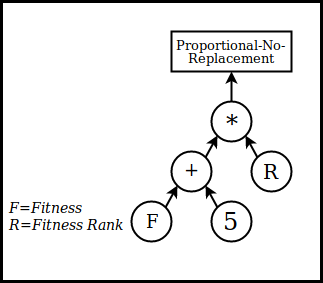
\includegraphics[width=0.25\textwidth]{example_eppsea_nolabel}
	\caption{Example of a generated selection function.}
	\label{fig:example_eppsea_nolabel}
\end{figure}

\subsection{Search Methodology}
\label{Methodology-Search Methodology}

We use a meta-EA to develop the selection functions described in Section~\ref{Methodology-Encoding Selection Functions}, treating each complete selection function as a member of a higher-order population. The quality of each selection function is determined by running CMA-ES on a suite of static training instances from a benchmark function class. The underlying EA utilizes the selection function in question, and keeps all other parameters constant. The performance of the underlying EA is used to determine the quality of a selection function; selection functions that enable the EA to perform better, with all other parameters constant, are considered to be ``higher-quality'' selection functions. The size of the GP-Trees is constrained using parsimony pressure.

When the meta-EA concludes, the CMA-ES utilizing the best selection function from the meta-EA is run on a set of separate testing instances from the same function class to test the generalization of the selection function's performance. If modified CMA-ES performs significantly better on the testing instances than the same EA using a standard selection function, then we can say that the evolved selection function successfully generalized to the function class of interest. 

The benchmark function classes used for the underlying EA are selected from the Comparing Continuous Optimizers (COCO) platform used for the GECCO Workshops on Real-Parameter Black-Box Optimization Benchmarking~\citep{cocobbob}. This benchmark set provides a suite of real-valued optimization problems. Each function class is offered in multiple dimensionalities, and for each dimension, multiple unique instances of the function class are present. By using several different instances of a given problem for a given dimensionality, we can test whether an increase in performance offered by a higher-quality selection function generalizes to other instances within the function class. We do this by using only some of the instances during the meta-EA to evaluate the quality of selection functions, then run CMA-ES utilizing the evolved selection function on the unused, unseen instances.

\section{Experimental Setup}
\label{Primary Experiments}
To test our methodology, we target the CMA-ES algorithm for improvement. We use the meta-EA to evolve a new method of selecting which of the sampled points to use for recalculating the search space mean. The individuals of the meta-EA each encode a single selection function in their genome, which modifies the mean-update functionality of CMA-ES. Rather than selecting the $\mu$ highest-fitness points, the encoded selection function selects a subset of all the sampled points, which are then ordered by fitness and used to update the mean. Once the mean is updated, all other state variables, such as the covariance matrix, are updated using the same methods as the unmodified CMA-ES.

To select benchmark functions for the CMA-ES, we use the 24 noiseless function classes in the COCO dataset. We use dimensionalities of 2, 3, 5, and 10, excluding 20 and 40 to save computational resources. The meta-EA is run separately for each combination of function class and dimensionality, using 6 of the instances for that function class and dimensionality to train the meta-EA and the rest of the available instances for testing generalization of the evolved selection function. For the parameters of CMA-ES, we use $\lambda=10 \times D$, $\mu = \lambda/2$, and $\sigma_i = 0.5$. The CMA-ES terminates on population convergence, after $10000 \times D$ evaluations, or after finding the solution to a function instance, as specified by the COCO benchmark platform.

When evaluating the performance of an evolved selection function to assign a fitness value to it, the fitness is taken as the proportion of the runs in which the modified CMA-ES reaches the global optimum, or moves close enough to it to meet the criteria to solve the function.

For each function instance in the testing set, we run the CMA-ES for 200 testing runs, both using the evolved selection function and unmodified. We then measure, for each testing instance, the proportion of runs which solved the function, in each case. 

\section{Results and Discussion}
\label{Results}

For the function classes 4, 6, 12, 17, 18, 19, 20, and 21, the CMA-ES modified with the evolved selection function solved the function instances at least 20 percent more often than the unmodified CMA-ES for at least one dimensionality. For the function classes 4 and 19, the success rate of CMA-ES increased by 20-30 percent when modified with the evolved selection function at $D=2$, but performed similarly to the unmodified CMA-ES at other dimensionalities. For function classes 20 and 21, a performance increase is seen on dimensionalities $D=2, 3,$ and $5$, but not $D=10$; curiously, the modified CMA-ES performs worse on function class 21 when $D=10$. For function classes 17 and 18, performance increases are seen for $D=2$ and $D=3$, with negligible performance differences on the other dimensionalities. Function class 22 sees about a 12 percent increase in solution rate on $D=2$, but negligible improvement for other dimensionalities. For function classes 6 and 12, performance is similar for $D=2, 3,$ and $5$, but for $D=10$, there is a significant performance increase: on function 6, the success rate increased from 0 percent to around 96 percent, and on function class 12, the success rate increased from 18-67 percent, varying across the function instances, to 100 percent for all function instances.

For the other function classes, there was no major difference between the success rate of the modified and unmodified CMA-ES. In a few cases, the modified CMA-ES performs marginally worse than the unmodified CMA-ES, but the difference in solution rate usually no more than 5 percent, and only 7.4 percent at most.

\subsection{Discussion of Results}
\label{resultsDiscussion}

We observed that evolving a new selection function for CMA-ES increased its solution quality on 6 of the 11 functions tested. In particular, we observed two cases with high dramatic improvements: the tests for COCO function classes 6 and 12 for dimensionality $D=10$. The five cases where no improvement was observed involved functions that were highly multimodal. It is likely, in these cases, that CMA-ES requires some other improvement aside from a new mean-update scheme to better learn and traverse the global structures of these functions. 

\section{Conclusions}
\label{Conclusion}
We hypothesized that a search through the space of selection functions could improve the performance of CMA-ES on a particular problem class by discovering a specialized selection function with which to modify the mean-update function of CMA-ES. We developed a representation of selection functions that utilizes a GP-Tree and selection method and used a meta-EA to search through the space of selection functions in this representation.

With this meta-EA, we have shown that it is possible to generate new selection functions, tuned to a particular benchmark function, that can enable CMA-ES to significantly outperform conventional selection functions on those functions. We have also shown that this performance increase from a custom selection algorithm will generalize to similar functions in the same function class. Therefore, if one expects to run CMA-ES, or any EA on many functions from the same function class, one might expect to gain a performance increase by doing some \textit{a priori} calculation to develop a specialized selection algorithm trained on instances of that function class. However, our experiments have also shown that, for certain functions, replacing only the selection function may not yield significant performance improvements, depending on the behavior of the search strategy and the nature of the function being optimized by the EA. 

\subsection{Comments on Methodology}
\label{Threats to Validity}
Although we strove to ensure the robustness of our methodology and experimental setup, there are some careful considerations that must be made when interpreting these results which may threaten the validity of our claims.

While we have shown improved performance on the benchmark functions tested, we still have yet to test this method on EAs run in real-world scenarios, and we do not yet know whether the supposed performance benefit is, in practice, enough to warrant the \textit{a priori} computation necessitated by our methods.

We chose CMA-ES as a testing target for extending our method to a more state-of-the-art method. However, the implementation of CMA-ES we used was fairly basic, lacking restarts in particular, and much research has been done on improved and alternative variants of CMA-ES. For certain problems, these newer variants may offer the same, or greater, performance increases as an evolved selection function. However, if these newer variants also use some selection function to update internal variables, as the basic implementation does, then evolving a new selection function for these newer variants could generate an even greater increase in performance; this opens up an avenue for future research.

\subsection{Future Work}
\label{Future Work}
The work presented in this paper opens a number of potential avenues for future research. Of primary concern is the fact that the meta-EA presented in this paper requires a large amount of \textit{a priori} computation to generate a high-quality selection function. While this computational cost may be worth it for EAs that will run on functions from the same function class many times, a more efficient method of finding good selection functions has a much greater potential to benefit EAs in general. Exploring a method of online learning could allow for the elimination of the expensive \textit{a priori} computation time, allowing specialized selection functions to be generated during the evolution.

The CMA-ES in our experiments was tuned to increase performance on the COCO benchmark function classes. While these functions are difficult and non-trivial to optimize for, they are entirely artificial, and the meta-EA has not yet been used to tune an EA for solving a real-world function class. A major next step for this work is to apply the meta-EA to real-world EAs that could benefit from new, specialized selection functions. Of particular interest are EAs that are expected to be run many times on functions from the same general function class, which would, over many runs, amortize the \textit{a priori} computation time required to tune the selection function.

Because the objective of this paper is similar to the work done to develop selection algorithms via Grammatical Evolution~\citep{lourencco2013selection} and register machines~\citep{woodward2011selection}, it remains to be seen which cases each method is more effective for, and a direct comparison of the methods on the same benchmark functions may yield more insight into which offers better performance benefits under certain conditions.

The framework of CMA-ES used was fairly basic, lacking features such as restarts. In addition, many techniques have been developed to improve CMA-ES, such as in $(1+1)$-CMA-ES~\citep{igel2006cmaes1plus1} and the Active CMA-ES~\citep{jastrebski2006activecmaes}. Evolving a specialized selection function for these new forms of CMA-ES may lead to even greater performance gains, or may not even be necessary for particular problem classes. Additionally, we only made efforts to improve the mean-update step of CMA-ES, which allowed to it gain increased performance in some, but not all, of the problem cases tested. Further experiments to tune the methods used for updating the other internal variables, such as evolution path, covariance matrix, and step-size, may lead to greater performance in more problem classes.

Adding additional available terminals to the GP-Tree increases the information available to the meta-EA, allowing it to potentially evolve more intelligent selection functions. In particular, there are no terminals that allow the selection function to have any internal persisting memory from generation to generation, such as the best fitness of past generations or which individuals have been selected previously. Additionally for EA's with sexual reproduction, or selection schemes involving individuals selected in pairs or groups, there is no terminal that measures two individuals relative to each other. This prevents the meta-EA from developing a selection function based on any information about an individual's mate, such as fitness, genome, etc. To add these terminals to the meta-EA, the selection function representation would need to be updated such that, when determining the desirability of an individual, the GP-Tree would take as input the information of some other individual to be selected for a similar purpose, such as recombination of the same child (for an EA with two-parent recombination) or selection for update of the same internal variable (for an Evolution Strategy such as CMA-ES).

The meta-EA parameters were manually tuned to allow for a high degree of exploration. A sensitivity analysis of these parameters, as well an investigation of parameter tuning/control, could lead to increased performance of the meta-EA.

\bibliographystyle{ACM-Reference-Format}
\bibliography{eppsea_GECCO2019_bibliography} 

\end{document}
